% DIVAS image processing workshop
% Image basics slides
%
% Mark M. Meysenburg
% 5/10/2017

\documentclass{beamer}

\mode<presentation> {

% set theme and color
\usetheme{CambridgeUS}
\usecolortheme{crane}
}

\usepackage{graphicx} % Allows including images

\usepackage{listings} % Allow sourcecode

\usepackage{hyperref} % Allow clickable hyperlinks

%----------------------------------------------------------------------------------------
%	TITLE PAGE AND FRONT MATTER
%----------------------------------------------------------------------------------------

\title[Image Basics]{IP Workshop: Image Basics} % The short title appears at the bottom of every slide, the full title is only on the title page

\author{Mark M. Meysenburg} % Your name
\institute[Doane DIVAS] % Your institution as it will appear on the bottom of every slide, may be shorthand to save space
{
Doane University \\ % Your institution for the title page
\medskip
\textit{mark.meysenburg@doane.edu} % Your email address
}
\date{\today} % Date, can be changed to a custom date

\begin{document}

\begin{frame}
\titlepage % Print the title page as the first slide
\end{frame}

\begin{frame}
\frametitle{Overview} 
\tableofcontents 
\end{frame}

%----------------------------------------------------------------------------------------
%	PRESENTATION SLIDES
%----------------------------------------------------------------------------------------

\section{Pixels}

\begin{frame}
	\frametitle{Introduction to pixels}

	\begin{itemize}
		\item Digital images are stored as rectangular arrays of hundreds, thousands, or millions of discrete``picture elements,'' otherwise known as pixels. Each pixel can be thought of as a single square point of colored light
		\item Each is all one color, but each pixel can have a different color from its neighbors. Viewed from a distance, these pixels seem to blend together to form the image we see
	\end{itemize}
\end{frame}

\begin{frame}
	\frametitle{Looking at pixels}

	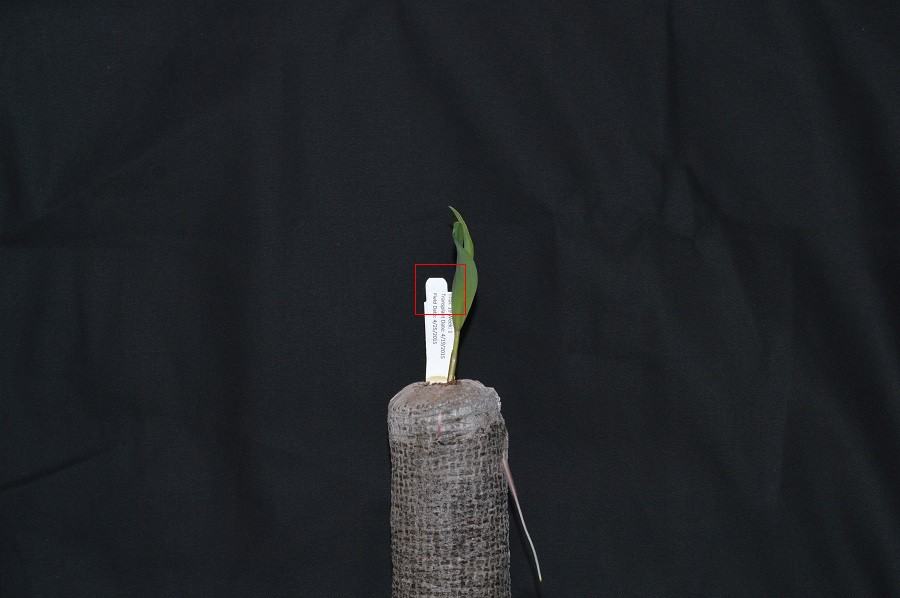
\includegraphics[width=0.95\textwidth]{../../fig/01-original.jpg}
\end{frame}

\begin{frame}
	\frametitle{Looking at pixels}

	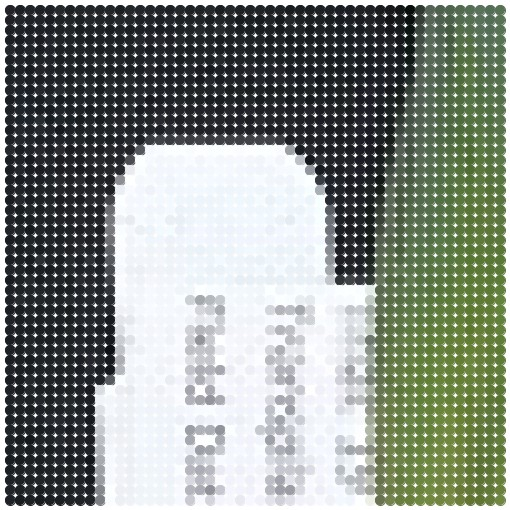
\includegraphics[width=0.95\textwidth]{../../fig/01-enlarged.jpg}
\end{frame}

\section{Coordinate system}

\begin{frame}
	\frametitle{Image coordinate system}

	\begin{itemize}
		\item We can access, examine, and / or change the color of any pixel we wish. To do this, we need some convention on how to access pixels individually; a way to give each one a name or an address of sort
		\item We use the {\em left-hand} coordinate system to specify the location of individual pixels
	\end{itemize}

\end{frame}

\begin{frame}
	\frametitle{Image coordinate system}

	{
	\centering
	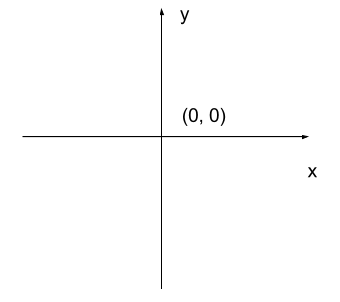
\includegraphics[width=0.45\textwidth]{../../fig/01-cartesian.png}%
	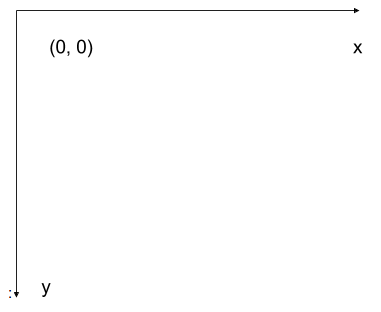
\includegraphics[width=0.45\textwidth]{../../fig/01-image-coordinates.png}
	}

\end{frame}

\begin{frame}
	\frametitle{Image coordinate system}

	\begin{center}
	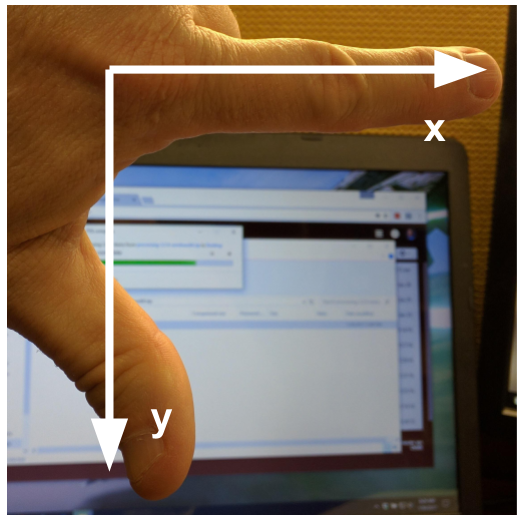
\includegraphics[width=0.6\textwidth]{../../fig/01-left-hand-coordinates.png}
	\end{center}

\end{frame}

\section{Color model}

\begin{frame}
	\frametitle{Introduction to color models}

	\begin{itemize}

		\item Digital images require some {\em color model} to create a broad range of colors from a small set of primary colors
		\item There are several different color models that are used for images, the most commonly occurring one is the additive red-green-blue ({\em RGB}) model
		\item In the RGB model, different intensities of red, green, and blue are combined to create the color for the image pixel

	\end{itemize}

\end{frame}

\begin{frame}
	\frametitle{Details of the RGB model}

	\begin{itemize}

		\item Each of the primary colors in the RGB model is often called a {\em channel}

		\item Usually, the amount of the primary color added is represented as an integer in the closed range [0, 255], giving 256 discrete values for that channel

		\begin{itemize}

			\item 256 comes from the number of bits used to represent the value

			\item Eight bits per channel gives the common {\em 24-bit color}

		\end{itemize}

		\item Any color in the RGB model can be expressed by a triplet of integers in [0, 255], representing the red, green, and blue channels, respectively. A larger number in a channel means that more of that primary color is present

		\item See, for example, \url{http://www.rapidtables.com/web/color/RGB_Color.htm}

	\end{itemize}

\end{frame}

\begin{frame}
	\frametitle{Details of the RGB model}

	\begin{itemize}

		\item With 24-bit color, we can represent $2^{24} = 16,777,216$ distinct colors

		\begin{itemize}

			\item The human eye can only distinguish approximately $10,000,000$ colors, so that seems to be plenty...
			
			\item ... unless you are doing science that looks at colors humans cannot distinguish!

		\end{itemize}

		\item Other common color depths:

		\begin{itemize}

			\item 8-bit color: 3 bits red, 3 bits green, 2 bits blue, for $8 \times 8 \times 4 = 256$ colors

			\item 16-bit color: 4 bits for each (plus 4 for {\em alpha}), giving $16 \times 16 \times 16 = 4,096$ colors

			\item 18-bit color: 6 bits for each, giving $64 \times 64 \times 64 = 262,144$ colors

		\end{itemize}

	\end{itemize}

\end{frame}

\section{Image formats}

\begin{frame}
	\frametitle{Image formats}

	\begin{itemize}

		\item Abstractly, we think of digital images as instances of {\em raster graphics}

		\begin{itemize}

			\item Rectangular arrays of pixels, with the color for each pixel specified by a RGB triplet

		\end{itemize}

		\item But, images are not necessarily stored in the computer, on disk, or transmitted over a network in that format

		\item There are several digital image file formats we might encounter:

		\begin{itemize}
	
			\item Device-Independent Bitmap (BMP), with {\tt .bmp} extension

			\item Joint Photographic Experts Group (JPEG), with {\tt .jpg} or {\tt .jpeg} extension

			\item Tagged Image File Format (TIFF), with {\tt .tif} extension

		\end{itemize}

	\end{itemize}
\end{frame}

\subsection{BMP images}

\begin{frame}
	\frametitle{BMP images}

	\begin{itemize}

		\item Closest file format to our raster graphics conceptualization

		\item Supports 8-, 16-, or 24-bit color

		\item Advantages:

		\begin{itemize}

			\item Simple file format

			\item High quality images

			\item Viewable by almost every system / application

		\end{itemize}

		\item Disadvantages:

		\begin{itemize}

			\item Images are not compressed, so file sizes are very large

		\end{itemize}

	\end{itemize}

\end{frame}

\subsection{Image compression}

\begin{frame}
	\frametitle{Image compression}

	Thought experiment: Imagine a $5,000 \times 5,000$ pixel image, composed of nothing but white pixels. How much storage space would be required to store the image?

	\begin{center}
	
\includegraphics[width=0.3\textwidth]{../../fig/01-white-square.jpg}
	\end{center}
\end{frame}

\begin{frame}
	\frametitle{Image compression}

	\begin{itemize}
	
		\item Since image files can be very large, various compression schemes exist for saving (perhaps approximately) the same information while using less space

		\item These compression techniques can be categorized as {\em lossless} or {\em lossy}

	\end{itemize}

\end{frame}

\begin{frame}
	\frametitle{Lossless compression}

	\begin{itemize}

		\item In lossless image compression, the computer applies some algorithm to the image, resulting in a file that is significantly smaller than the uncompressed file equivalent would be. Then, when we wish to load and view or process the image, our program reads the compressed file, and reverses the compression process, resulting in an image that is identical to the original. Nothing is lost in the process – hence the term ``lossless.''

		\item See the white-square-making program
	\end{itemize}
\end{frame}

\begin{frame}
	\frametitle{Lossy compression}

	\begin{itemize}

		\item Lossy compression takes the original image and discards some of the detail in it, resulting in a smaller file format. The goal is to only throw away detail that someone viewing the image would not notice. Many lossy compression schemes have adjustable levels of compression, so that the image creator can choose the amount of detail that is lost. The more detail that is sacrificed, the smaller the image files will be -- but of course, the detail and richness of the image will be lower as well.

		\item It is important to understand that once an image is saved in a lossy compression format, the lost detail is just that -- lost. I.e., unlike lossless formats, given an image saved in a lossy format, there is no way to reconstruct the original image in a byte-by-byte manner.

	\end{itemize}

\end{frame}

\begin{frame}
	\frametitle{Lossy compression example}

	\begin{center}
	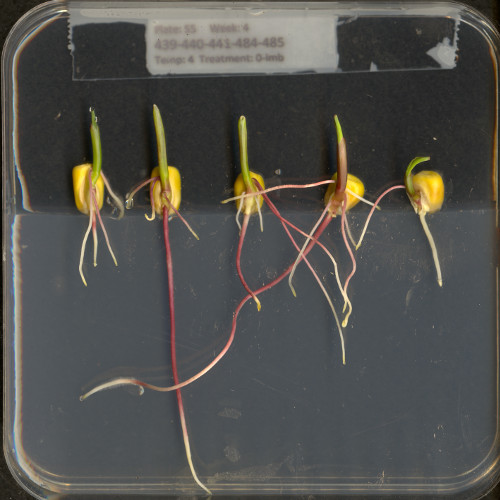
\includegraphics[width=0.5\textwidth]{../../fig/01-quality-orig.jpg}
	\end{center}

\end{frame}

\begin{frame}
	\frametitle{Lossy compression example}

	\begin{center}
	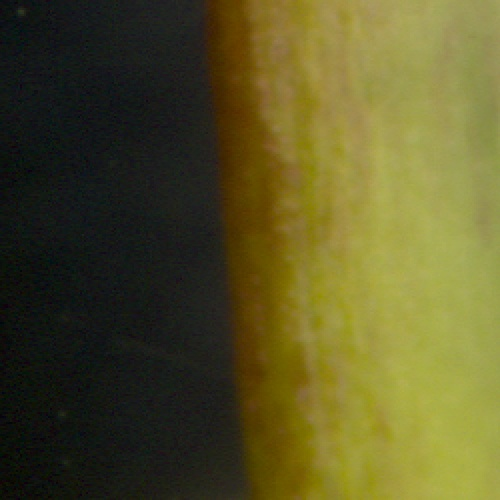
\includegraphics[width=0.5\textwidth]{../../fig/01-quality-tif.jpg}
	\end{center}

\end{frame}

\begin{frame}
	\frametitle{Lossy compression example}

	\begin{center}
	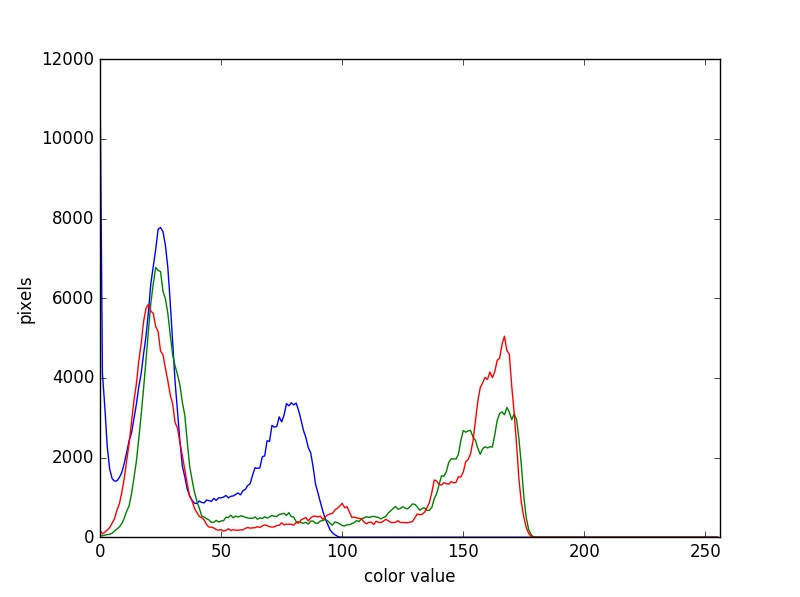
\includegraphics[width=0.5\textwidth]{../../fig/01-quality-tif-histogram.jpeg}
	\end{center}

\end{frame}

\begin{frame}
	\frametitle{Lossy compression example}

	\begin{center}
	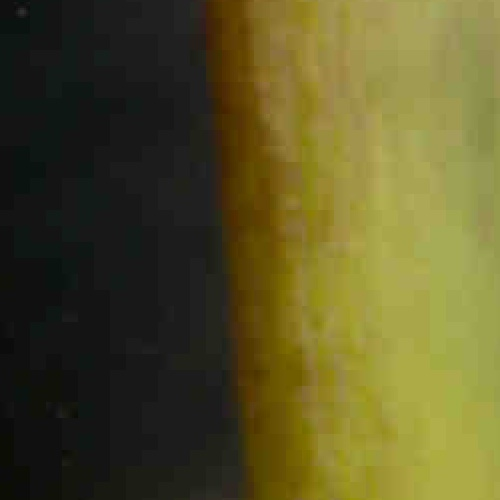
\includegraphics[width=0.5\textwidth]{../../fig/01-quality-jpg.jpg}
	\end{center}

\end{frame}

\begin{frame}
	\frametitle{Lossy compression example}

	\begin{center}
	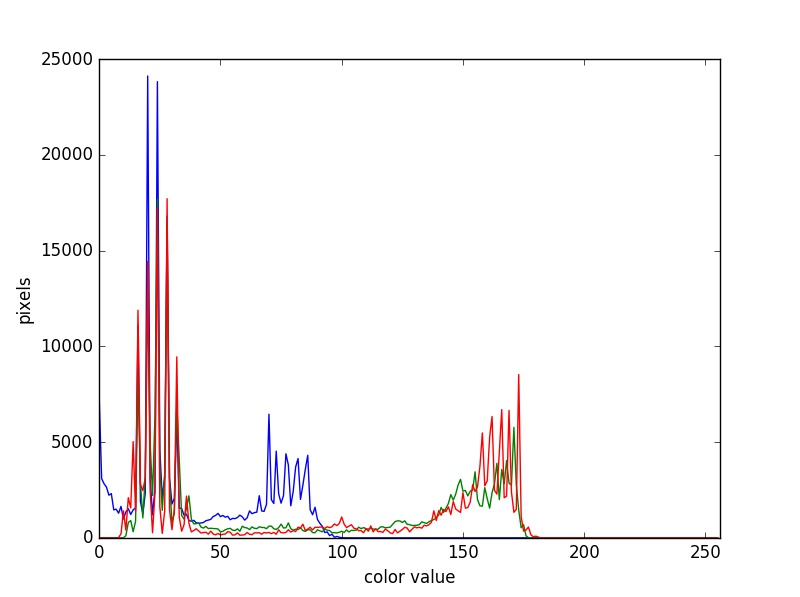
\includegraphics[width=0.5\textwidth]{../../fig/01-quality-jpg-histogram.jpeg}
	\end{center}

\end{frame}

\subsection{JPEG images}

\begin{frame}
	\frametitle{JPEG images}

	\begin{itemize}

		\item Most common digital image format

		\item Uses tunable, lossy compression

		\item 24-bit color depth

		\item Advantages:

		\begin{itemize}

			\item Viewable by almost every system / application

		\end{itemize}

		\item Disadvantages:

		\begin{itemize}

			\item Lossy compression may remove needed detail from images

		\end{itemize}

		\item Rule of thumb: If you are using JPEG images, set the compression rate low to preserve as much detail as possible

	\end{itemize}

\end{frame}

\subsection{TIFF images}

\begin{frame}
	\frametitle{TIFF images}

	\begin{itemize}

		\item Popular with publishers, graphics designers, and photographers

		\item Can be uncompressed, or compressed using either lossless or lossy compression schemes

		\item Advantages:

		\begin{itemize}

			\item High quality with small file size (if lossless compression is selected)

		\end{itemize}

		\item Disadvantages:

		\begin{itemize}

			\item High file size or loss of detail, depending on compression options

			\item Not universally supported in all systems / applications

		\end{itemize}

	\end{itemize}

\end{frame}

\section{Image metadata}

\begin{frame}

	\frametitle{Image metadata}

	\begin{itemize}

		\item {\em Image metadata} is textual information that is contained within an image file, but not normally shown when the image is viewed

		\item Metadata holds information about the image itself, such as when the image was captured, where it was captured, what type of camera was used and with what settings, etc.

		\item Users can also edit metadata, adding custom information to images

		\item JPEG and TIFF images support the inclusion of metadata in images

	\end{itemize}
\end{frame}

\begin{frame}
	\frametitle{Metadata example}

	Using ImageJ, examine the metadata for this image.

	\begin{center}

		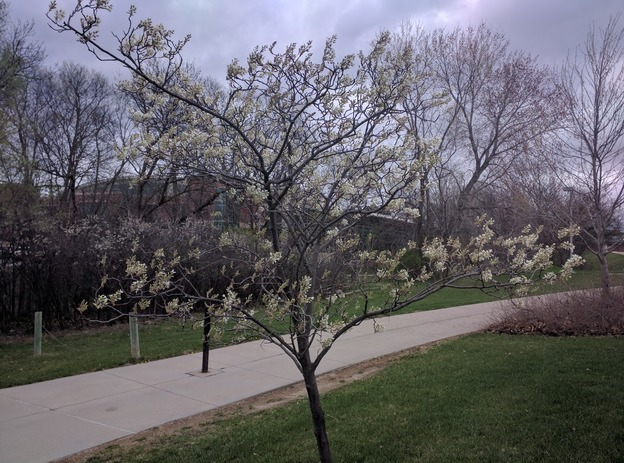
\includegraphics[width=0.6\textwidth]{../../fig/01-metadata-before.jpg}

	\end{center}

\end{frame}

\end{document}


